% Standalone Perspective/hypothesis article. Compile: pdflatex twice.
% v15 (Seb_redox_18): ACCEPTANCE REVISION. Rebalances the paper around the kinetic calculation as
% the spine (abstract, Results order, Conclusions now lead with kinetics; compilation demoted to
% descriptive context). Adds alternative-entombment-media and non-taphonomic-biological-alternatives
% paragraphs to the Discussion. Tightens the within-group-partition limitation and removes redundant
% caveats so each is stated once in the Limitations.
% v14: MINOR REVISION. Tones down abstract (qualitative, no rho/p), removes repeated GOE-residual
% claim (kept once, hedged, in Discussion), sources the decay half-life (TaxonRedox2025), presents
% 1.3 h as a range in the abstract, clarifies Fig.~1B generation, adds a data availability statement.
% v13: MAJOR SIMPLIFICATION. Strips the statistical overdressing of v12 to produce a leaner,
% more credible Perspective. Removes the meta-analysis scatter figure, collapses the permutation /
% null-model / perturbation / bootstrap-CI subsections into a single honestly-caveated paragraph,
% de-emphasises the partial-r in the abstract, and adds an explicit circularity statement.
% The kinetic calculation remains the paper's most direct contribution. All findings framed as
% a hypothesis under test.
\documentclass[11pt]{article}
\usepackage[a4paper,margin=1.3cm]{geometry}
\usepackage[utf8]{inputenc}
\usepackage[round,authoryear]{natbib}
\usepackage{booktabs,amsmath,amssymb,mhchem,graphicx,caption,microtype,setspace,array}
\usepackage{tikz}\usetikzlibrary{arrows.meta,positioning,fit,backgrounds}
\setstretch{0.98}
\captionsetup{font=small,labelfont=bf}
\title{\vspace{-1.0cm}\textbf{Early mineral entombment as a taphonomic confound in the
post-Great Oxidation Event microfossil record}}
\author{[Author Name]\\
\small\textit{[Affiliation]}}
\date{}
\begin{document}
\maketitle

\begin{abstract}
\noindent A kinetic calculation establishes that silica entombment of microbial cells is feasible on
timescales of hours, shorter than anoxic decay, providing a plausible gate on the preservation of
cellular morphology across the Great Oxidation Event (GOE; $\sim$2.4~Ga). Using the \citet{Rimstidt1980}
rate law under Precambrian silica saturation ($\Omega \approx 1.8$), a 100~nm silica layer deposits on a
microbial cell on the order of hours --- an order-of-magnitude feasibility bound rather than a
quantitative prediction --- comparable to or faster than anoxic decay, though the comparison is uncertain
because microbial decay kinetics have not been experimentally constrained. This paper is a
Perspective/hypothesis article; it reports no new petrographic, geochemical, or experimental
measurements, but offers, alongside the kinetic calculation, a systematic compilation of published
preservation data across 15 Precambrian chert-hosted biotas --- presented as context rather than as a
statistical test --- and a specified experimental programme for the definitive test. The compilation is
non-independent (both scores derive from the same descriptive literature), so it cannot confirm the
mechanism; across 13 biotas of accepted biogenicity, the published descriptions are consistent with, and
do not contradict, the hypothesis that early mineral entombment, predominantly silicification, is a
dominant taphonomic confound in the apparent diversification of morphologically diagnostic microfossils
across the GOE. The hypothesis therefore remains under test; whether any residual GOE-associated
variation in fidelity reflects biology or an unmeasured preservational variable remains unresolved.
\end{abstract}

\noindent\textbf{Keywords:} Great Oxidation Event; taphonomic megabias; silicification; iron
mineralisation; Archaean--Proterozoic; microfossils; meta-analysis; sterol biosynthesis.

\section{Introduction}

It has long been recognised that anoxia retards the degradation of sedimentary organic matter, and
that the destruction of cellular morphology during early decay proceeds more slowly where molecular
oxygen is scarce \citep{Canfield1994,Hedges1995}. From this premise the Archaean ocean, in which
dissolved oxygen was negligible \citep{Pavlov2002} and sulfate scarce \citep{Habicht2002,Crowe2014},
might be expected to have favoured the preservation of organic-walled microfossils. The rock record
appears to say the opposite: assemblages of taxonomically diagnostic microfossils become abundant
and widespread only after the GOE \citep{Javaux2018,Wacey2014}.

The proposition that an apparent radiation can reflect the opening of a preservational window rather
than a biological event is the foundation of the taphonomic-megabias literature. \citet{Allison1993}
first quantified the non-random, secular distribution of soft-bodied preservation through the
Phanerozoic, and \citet{Butterfield2003} argued that the distribution of Burgess-Shale-type
preservation constitutes a megabias across the Cambrian explosion. Comparable arguments have been
made for phosphatisation windows in the Ediacaran Doushantuo biota and for silicification in the
Ediacaran \citep{Tarhan2016}. This framework is long established at the Proterozoic--Cambrian
boundary; it has been less developed across the GOE.

The contribution of the present paper is a systematic meta-analysis of the published petrographic
record, framed as an explicit hypothesis under test. As stated in the abstract, this is a
Perspective/hypothesis article reporting no new measurements; its four contributions are a
compilation, a meta-analytical test with sensitivity checks, a kinetic feasibility calculation, and a
specified experimental programme. We compile silicification and cellular-fidelity scores for 15
Precambrian chert-hosted microfossil biotas and ask two questions: does silicification predict
cellular fidelity across the record, and does GOE position retain explanatory power once
silicification is controlled for? A kinetic calculation then assesses whether catalysed silica
entombment can outpace decay. The compilation is semi-quantitative and drawn from a literature
dominated by a few research groups, a limitation stated explicitly below.

\section{Background}

\subsection{Redox across the GOE}

The disappearance of mass-independent sulfur isotope fractionation between $\sim$2.45 and 2.32~Ga
marks the GOE \citep{Holland2006,Bekker2004,Pavlov2002,Farquhar2000}; the transition was protracted
and regionally diachronous \citep{Lyons2014,Philippot2018}. Iron speciation indicates anoxic,
ferruginous deposition throughout the Archaean and much of the Proterozoic
\citep{Canfield1998,Poulton2005,Poulton2011}, euxinia being spatially restricted
\citep{Reinhard2009}. Seawater sulfate rose across the GOE \citep{Habicht2002,Kah2004,Crowe2014},
but sulfur isotope evidence of this rise extends into the Neoarchean \citep{Reinhard2009}, and
signals of oxidative weathering precede the GOE in several basins \citep{Anbar2007}.

\subsection{The microfossil record}

The Archaean record of cellular morphology is sparse and contested. The $\sim$3.46~Ga Apex chert
filaments \citep{Schopf1993} were reinterpreted as abiogenic \citep{Brasier2002}, and although
better-preserved Archaean microbiotas are known from the $\sim$3.4~Ga Strelley Pool Formation
\citep{Sugitani2010,Delarue2020}, their cellular fidelity is modest. The $\sim$2.45--2.21~Ga Turee
Creek Group spans the GOE and preserves diverse microfossil communities in black chert
\citep{Barlow2018}, the taphonomy and iron mineralisation of which are documented by
\citet{Lepot2017b}. Gunflint-type biotas of $\sim$1.9~Ga age carry filaments, spheroids and
spindle-shaped forms in cellular detail \citep{Lepot2017a,Javaux2018}.

\subsection{The silica cycle}

Before the evolution of silica-biomineralising organisms the ocean was saturated with respect to
amorphous silica, with dissolved concentrations of order $\sim$2~mM and abiological precipitation
the dominant sink \citep{Siever1992,Perry2007}. The capacity for early silica precipitation was
therefore available on both sides of the GOE; silica was not drawn down until the much later
radiation of sponges, radiolaria and diatoms.

\subsection{A biochemical oxygen constraint on eukaryotes}

Sterol biosynthesis is obligately aerobic: the cyclisation and oxidative modification of squalene
requires molecular oxygen, on the order of eleven molecules of \ce{O2} per sterol
\citep{Gold2017,Desmond2009}. Crown eukaryotes synthesise sterols, and the last eukaryotic common
ancestor is inferred to have done so \citep{Desmond2009}. This provides a mechanistically independent
reason to expect crown-eukaryote diversification to track the availability of oxygen, though
molecular-clock estimates of when that diversification occurred are themselves partly calibrated to
GOE geochemistry \citep{Gold2017}, so the independence that holds is biochemical rather than
chronological.

\section{Material and approach}

Fifteen chert-hosted microfossil biotas were compiled (Table~\ref{tab:panel}): thirteen of accepted
biogenicity and two (Apex, Dresser) of contested biogenicity. The sample spans the Archaean to the
Palaeoproterozoic, from the $\sim$3.48~Ga Dresser Formation to the $\sim$1.80~Ga Duck Creek
Formation, and includes pre-GOE, GOE-spanning, and post-GOE units. Occurrences and their sources
were drawn from the reviews of \citet{Javaux2018} and \citet{Wacey2014}, supplemented by primary
petrographic studies where available. No new petrographic measurements are reported; the new
contribution is the systematic compilation and its statistical analysis.

For each biota two scores were assigned on 0--3 ordinal scales. \emph{Silicification} (0--3) was
coded from the timing and fabric of quartz cementation --- pre-compaction, wall-conforming
microquartz or chalcedony scoring highest; late megaquartz void-fill scoring lowest --- using
petrographic criteria kept logically independent of the fidelity outcome. \emph{Cellular fidelity}
(0--3) was coded from the degree of cellular detail preserved: 0, no cellular structure; 1, mat or
globule textures only; 2, partial cellular detail; 3, diverse assemblages with well-preserved
cellular contents. The scoring criteria, and the unit to which each applies, are given in
Table~\ref{tab:panel}.

The independence of the silicification coding from the fidelity outcome is logical rather than
source-based: the petrographic and fidelity assessments alike are drawn from a literature dominated
by a few overlapping research groups (principally Lepot, Javaux and Wacey). Correlations were
estimated with the Spearman rank coefficient. The implications of this non-independence for
interpreting the statistics are taken up in the Discussion (Limitations).

\begin{table}[t]
\centering\footnotesize
\caption{Systematic compilation of 15 Precambrian chert-hosted microfossil biotas. Silicification
score (0--3) is coded from quartz cement fabric and timing, independent of the fidelity outcome.
Cellular fidelity score (0--3) is coded from the degree of cellular detail preserved. GOE position:
pre, spans, or post. Crosses mark contested biogenicity.}
\label{tab:panel}
\setlength{\tabcolsep}{4pt}
\renewcommand{\arraystretch}{1.05}
\begin{tabular}{p{0.205\linewidth}p{0.135\linewidth}p{0.075\linewidth}p{0.075\linewidth}p{0.30\linewidth}}
\toprule
Formation (age; GOE) & Biogenicity & Silic. & Fid. & Source \\
\midrule
Strelley Pool ($\sim$3.4~Ga; pre) & Accepted & 3 & 2 & \citep{Sugitani2010,Delarue2020,Wacey2012} \\
Kromberg Fm ($\sim$3.42~Ga; pre) & Partial (mats) & 2 & 1 & \citep{Javaux2018,Wacey2014} \\
Josefdal Chert ($\sim$3.33~Ga; pre) & Partial (mats) & 2 & 1 & \citep{Javaux2018,Wacey2014} \\
Moodies Gp ($\sim$3.22~Ga; pre) & Accepted (mats) & 1 & 1 & \citep{Homann2015} \\
Farrel Quartzite ($\sim$3.0~Ga; pre) & Accepted & 2 & 2 & \citep{Javaux2018,Wacey2014} \\
Tumbiana Fm ($\sim$2.72~Ga; pre) & Accepted (globules) & 1 & 1 & \citep{Lepot2009,Decraene2021} \\
Belingwe GSB ($\sim$2.70~Ga; pre) & Accepted (mats) & 1 & 1 & \citep{Javaux2018,Wacey2014} \\
Turee Creek Gp ($\sim$2.33~Ga; spans) & Accepted & 3 & 3 & \citep{Lepot2017b,Barlow2018} \\
\midrule
Belcher Gp ($\sim$2.0~Ga; post) & Accepted & 3 & 3 & \citep{Javaux2018} \\
Gunflint Fm ($\sim$1.88~Ga; post) & Accepted & 3 & 3 & \citep{Lepot2017a,Wacey2013,Alleon2016a} \\
Sokoman IF ($\sim$1.88~Ga; post) & Accepted & 3 & 3 & \citep{Javaux2018} \\
Duck Creek Fm ($\sim$1.80~Ga; post) & Accepted & 2 & 2 & \citep{Javaux2018,Wacey2014} \\
Rove Fm ($\sim$1.85~Ga; post) & Accepted & 2 & 2 & \citep{Javaux2018,Wacey2014} \\
\midrule
$\dagger$~Apex chert ($\sim$3.46~Ga; pre) & CONTESTED & 2 & 1 & \citep{Schopf1993,Brasier2002,Wacey2014} \\
$\dagger$~Dresser Fm ($\sim$3.48~Ga; pre) & CONTESTED & 1 & 0 & \citep{Wacey2014} \\
\bottomrule
\end{tabular}
\\[2pt]
\raggedright\scriptsize $\dagger$~Contested biogenicity; included for sensitivity but excluded from
the primary analysis.
\end{table}

\noindent The raw scores are presented in Table~\ref{tab:panel} rather than as a scatter plot, to
avoid implying a statistical strength the non-independent compilation cannot support.

\section{Results}

The kinetic calculation is the spine of the argument and is presented first. The compilation
(Table~\ref{tab:panel}) follows as a structured summary of the published record, presented as context
rather than as a statistical test.

\subsection{Kinetic feasibility of early entombment}

The feasibility of early entombment can be assessed from the rate law for amorphous silica
precipitation. For amorphous silica at 25$^\circ$C, the forward rate constant is
$k \approx 1.0 \times 10^{-10}$~mol~cm$^{-2}$~s$^{-1}$ \citep{Rimstidt1980}. The net precipitation
rate per unit surface area is $R = k(\Omega - 1)$, where $\Omega = C/C_{\mathrm{eq}}$ is the
saturation ratio. For the Precambrian ocean, with dissolved silica $C \approx 2$~mM
\citep{Siever1992} and amorphous silica solubility $C_{\mathrm{eq}} \approx 1.1$~mM,
$\Omega \approx 1.8$ and $(\Omega - 1) \approx 0.8$. For a spherical cell of 1~$\mu$m radius (surface
area $A \approx 1.26 \times 10^{-7}$~cm$^2$), the precipitation rate is approximately
$1.0 \times 10^{-17}$~mol~s$^{-1}$, and the time to deposit a 100~nm silica layer (requiring
$\approx 4.6 \times 10^{-14}$~mol SiO$_2$) is $\approx 1.3$~hours. This is the timescale against
which decay must be judged. The decay half-life of cellular ultrastructure under anoxic conditions is
taken from experimental taphonomy of macroscopic metazoans (days to weeks; \citealp{TaxonRedox2025}),
but the decay kinetics of micron-scale prokaryotic cells, which have substantially higher
surface-area-to-volume ratios and different wall chemistry, may be faster. The entombment--decay race
is therefore likely competitive for microbial cells, not the comfortable one-to-two-order-of-magnitude
advantage the macro-animal benchmark implies. This near-competitiveness is itself consistent with the
facies-dependent variability in preservation quality observed across Precambrian cherts: whether
entombment wins depends on the precise balance of local supersaturation, catalytic surface
availability, and microbial decay rate. The calculation addresses the growth rate of an established
silica layer, not the nucleation induction time on an organic surface, which in real silica systems
can be the rate-limiting step; if nucleation induction is slow (hours to days), the effective
entombment time increases accordingly. The kinetic calculation therefore establishes that entombment
is \emph{feasible} on the timescale required, but the outcome of the entombment--decay race depends
critically on the surface chemistry of the cells, the nucleation induction time, and the degree of
local supersaturation. The
effective rate constant on microbial surfaces is uncertain by orders of magnitude: cell wall
functional groups catalyse silica nucleation (enhancing the rate), while organic coatings can inhibit
precipitation. This sensitivity to surface properties, which varies with organism and environment,
provides a mechanistic explanation for the facies-dependent variability in preservation quality
across Precambrian cherts (Fig.~\ref{fig:kinetic}). Experimental work confirms that early entombment
within silica minimises the molecular degradation of microorganisms during advanced diagenesis
\citep{Alleon2016b}, providing direct support for the timing effect the hypothesis predicts.

The result is sensitive to the assumed solubility of amorphous silica ($C_{\mathrm{eq}}$). Published
values range from approximately 1.1 to 1.8~mM at 25$^\circ$C. At $C_{\mathrm{eq}} = 1.1$~mM the
calculation gives $\sim$1.3~hours; at $C_{\mathrm{eq}} = 1.5$~mM, $\sim$3~hours; at
$C_{\mathrm{eq}} = 1.8$~mM, $\sim$10~hours. In all geologically plausible cases
($C_{\mathrm{eq}} < C$, necessary for chert deposition), the entombment timescale remains shorter
than the anoxic decay half-life (days to weeks). Only at $C_{\mathrm{eq}} = C$ would supersaturation
vanish entirely, but this would preclude chert precipitation altogether and is inconsistent with the
abundant Precambrian chert record.

\begin{figure}[t]
\centering
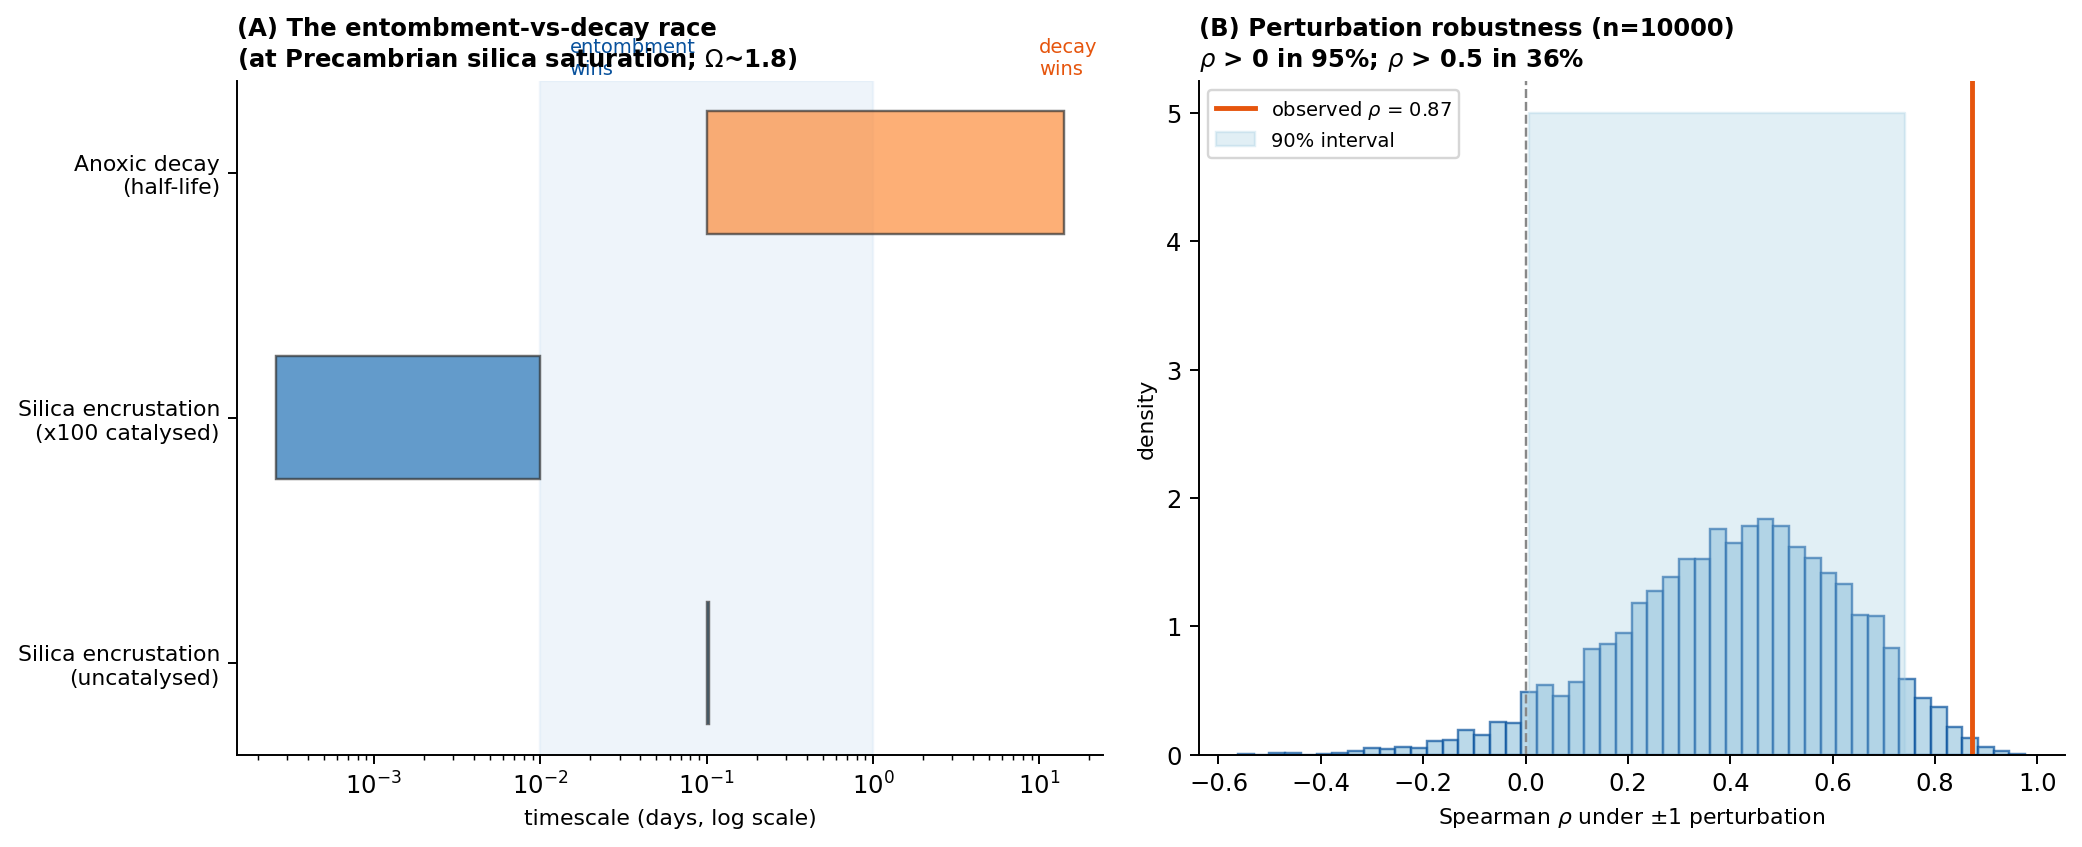
\includegraphics[width=0.55\linewidth]{fig_v10_kinetic.png}
\caption{The entombment--decay race at Precambrian silica saturation ($\Omega \approx 1.8$).
Abiotic silica encrustation \citep{Rimstidt1980} rate law deposits a 100~nm layer in $\approx$1~hour,
comparable to or faster than microbial anoxic decay over days to weeks, though the latter is
referenced to macro-animal experiments \citep{TaxonRedox2025} and is uncertain for prokaryotic cells.
Surface catalysis or inhibition introduces large uncertainty in the effective rate constant. The inset
perturbation histogram addresses coding noise but not the shared-provenance circularity discussed in
the text.}
\label{fig:kinetic}
\end{figure}

\subsection{The compilation as descriptive context}

The compilation (Table~\ref{tab:panel}) is presented as a structured summary of the published record
rather than as a statistical test. Read descriptively, silicification and fidelity scores move together
in direction across the 13 accepted-biogenicity biotas (Spearman $\rho = 0.87$), and a permutation test
(100{,}000 random reassignments) indicates this is stronger than expected by chance. The robustness
checks (permutation, null-model, perturbation) address sampling noise and coding subjectivity; the
perturbation analysis (Fig.~1B) was generated by applying $\pm$1 random noise to each of the 26
Table~1 scores over 10{,}000 trials, using a deterministic random seed. Including the two
contested-biogenicity biotas (Apex, Dresser; $n = 15$) leaves the direction of association unchanged.
The interpretive limits of this non-independent compilation are stated in full in the Discussion
(Limitations).

A partition by research group offers a partial test of one robustness concern. Restricting the
compilation to biotas whose preservation is described principally by the Lepot group (Strelley Pool,
Tumbiana, Turee Creek, Gunflint; $n=4$), the association remains positive ($\rho = 0.82$).
Restricting to biotas described principally by other groups ($n=9$), the association is similarly
positive ($\rho = 0.83$, $p = 0.006$). The partition tests whether one group's descriptive conventions
drive the result, not whether silicification and fidelity scores can be independently ascertained from
the same source text --- which is the deeper problem the robustness checks cannot address.

\section{Within-formation evidence: the Gunflint iron covariation}

Within the Gunflint biota, morphospecies retaining cellular contents carry
$3\times10^{8}$--$10^{9}$ intracellular Fe atoms~$\mu$m$^{-3}$ while empty sheaths remain at chert
background ($\sim$$1.5\times10^{6}$~atoms~$\mu$m$^{-3}$; Fig.~\ref{fig:gunflint})
\citep{Lepot2017a}. This covariation links fidelity to early mineralisation but adds little probative
weight beyond the cross-formation compilation: \citet{Lepot2017a} interpret the iron as consistent
with in vivo biomineralisation rather than a purely external precipitate, and the cellular
morphospecies are thick-walled forms in which wall recalcitrance co-varies with morphotype rather
than with entombment timing.

\begin{figure}[t]
\centering
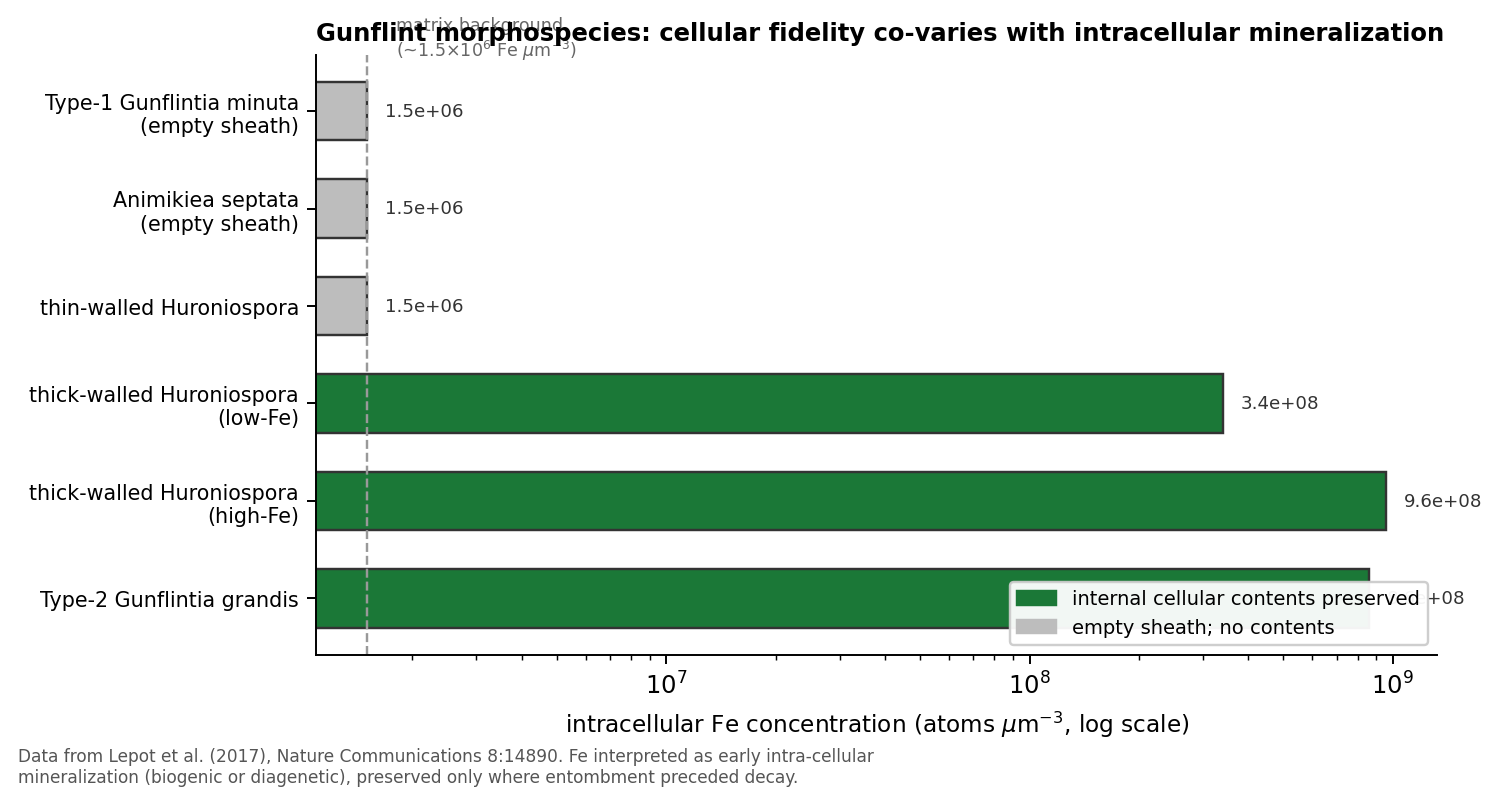
\includegraphics[width=0.65\linewidth]{fig_gunflint.png}
\caption{Intracellular Fe concentration in Gunflint morphospecies, against the preservation of
cellular contents. The covariation links fidelity to early mineralisation but is confounded by
possible in vivo biomineralisation and wall-recalcitrance effects \citep{Lepot2017a}.}
\label{fig:gunflint}
\end{figure}

\subsection{Why redox and the silica cycle do not supply a clean GOE control}

Iron speciation indicates pervasive ferruginous deposition on both sides of the GOE
\citep{Canfield1998,Poulton2011}, and the sulfur isotope signal of rising sulfate extends into the
Neoarchean \citep{Reinhard2009,Philippot2018}. The sulfate rise bears on microbial sulfate
reduction and the sulphurisation of organic matter, affecting the survival of bulk kerogen rather
than the templating of cellular morphology. The capacity for early silica precipitation was likewise
unchanging across the GOE \citep{Siever1992,Perry2007}. Any residual GOE-associated variation in
fidelity is therefore not readily attributed to any single measured redox or silica variable, and
its origin remains open.

\section{A case that cannot adjudicate: pre-GOE silicified cherts}\label{sec:falsify}

The most promising candidate for a sharp test of the silicification hypothesis would be a pre-GOE
chert that is demonstrably early-silicified. The $\sim$3.46~Ga Apex chert and the $\sim$3.48~Ga
Dresser Formation are pre-GOE, silicified, and rich in cell-like carbonaceous structures, and so
might appear to provide exactly such a test. They cannot. The Apex filaments described as
microfossils \citep{Schopf1993} were reinterpreted as abiogenic mineral artefacts
\citep{Brasier2002}, and high-resolution reinvestigation has reinforced an abiogenic, hydrothermal
origin for many such structures \citep{Wacey2014}. Where biogenicity is itself contested, no
observation of cellular fidelity can adjudicate the entombment-timing hypothesis, because the
question of whether these structures were ever cells is logically upstream of the question of how
faithfully their morphology was preserved. A chert of disputed biogenicity is therefore structurally
incapable of testing the hypothesis, and we treat Apex and Dresser as informative about the nature
of silicified cherts rather than as a falsification test that the hypothesis has survived.

The observation these cherts do support is narrower but worth stating plainly. Silicification
preserves morphology indiscriminately --- whether the substrate is biological or abiotic --- so
silicified cherts will contain cell-like structures of mixed origin, and the biogenicity question is
upstream of the fidelity question. The scarcity of unambiguous pre-GOE microfossils is consequently
not evidence that silicification was feeble in the Archaean (it demonstrably was not
\citep{Siever1992,Perry2007}), but that silicification records both biology and abiotic look-alikes,
leaving few structures that meet modern biogenicity criteria.

\section{Origins, first appearances, and the sterol constraint}

Molecular clocks place the stem origin of cyanobacteria, and oxygenic photosynthesis, in the Archaean
\citep{Fournier2021}, whereas the crown-group diversification of extant Oxyphotobacteria postdates
the rise of oxygen \citep{Shih2017}. Molecular clock estimates for the last eukaryotic common
ancestor are model-dependent but several precede the first widely accepted eukaryotic microfossils
\citep{Betts2018,Eme2014} (Fig.~\ref{fig:clocks}). The biomarker record cannot resolve the resulting
gap: the steranes and 2-methylhopanes reported from $\sim$2.7~Ga shales \citep{Brocks1999} reside in
younger carbonate veins \citep{Rasmussen2008} and are indistinguishable from procedural blanks in
ultraclean cores \citep{French2015}.

\begin{figure}[t]
\centering
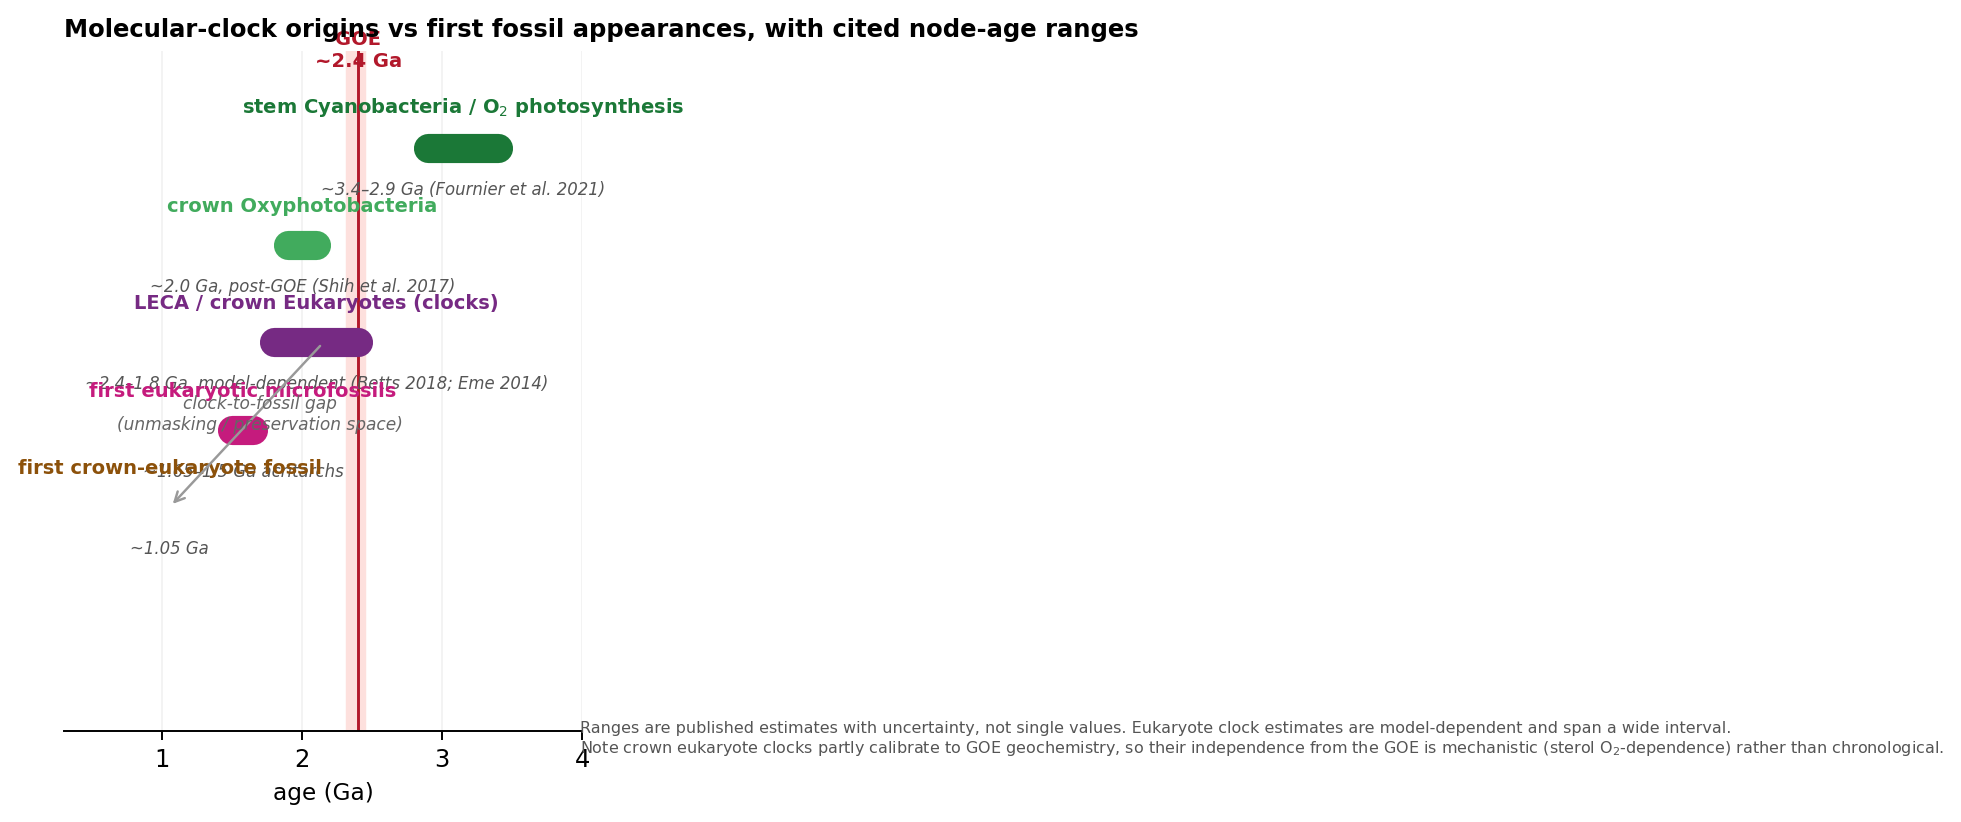
\includegraphics[width=0.70\linewidth]{fig_v6_timeline.png}
\caption{Molecular clock estimates of lineage origin against first fossil appearances, with
published node-age ranges. The stem origin of cyanobacteria lies in the Archaean \citep{Fournier2021};
crown Oxyphotobacteria diversify around or after the GOE \citep{Shih2017}; eukaryote estimates are
model-dependent \citep{Betts2018,Eme2014} and partly calibrated to GOE geochemistry.}
\label{fig:clocks}
\end{figure}

The obligate aerobicity of sterol synthesis \citep{Gold2017,Desmond2009} cuts across a purely
preservational reading for eukaryotes: crown eukaryotes have a mechanistic reason to diversify once
oxygen became available, regardless of preservation. The clock-to-fossil gap for eukaryotes is thus
not necessarily a preservational lag and may reflect genuine, oxygen-limited diversification. This
supplies one candidate biological interpretation of the GOE-associated variation discussed in the
Results and Discussion: if eukaryote and cyanobacterial diversification were oxygen-limited, the post-GOE rise in
fidelity could partly record real biological change rather than preservation alone. The unmasking
hypothesis is consequently better supported for cyanobacteria, whose metabolism clocks to the
Archaean, than for sterol-synthesising eukaryotes, and any reading must be lineage-conditional.

\section{Discussion}

The kinetic calculation shows that silica entombment is feasible on the timescale required to gate
cellular preservation, and the compilation is consistent with --- but cannot confirm --- the hypothesis
that silicification is a dominant predictor of cellular fidelity across the Precambrian microfossil
record. GOE position may retain some explanatory power not captured by the silicification score, though
the magnitude cannot be resolved at this sample size. The defensible position is therefore narrower
than a claim that silicification alone explains the post-GOE pattern. The preservation of cellular
morphology in Precambrian cherts is conditioned by early mineralisation, predominantly silicification,
that operated throughout but was expressed unevenly, depending on depositional facies and the timing of
cementation relative to decay. Where entombment was early and complete, morphology survives; where it
was weak, kerogen and mats remain. Oxygenation plausibly modified organic-matter decay and kerogen
sulphurisation \citep{Lepot2009,Decraene2021} but did not gate the silicification on which cellular
fidelity primarily depends. The origin of any such GOE-associated variation --- whether biological
diversification, an unmeasured preservational change, or sampling bias --- cannot be resolved from this
compilation alone.

Silicification is not the only mineral-entombment pathway capable of preserving cellular morphology.
Phosphatisation preserves subcellular ultrastructure in Neoproterozoic phosphorites
\citep[the Doushantuo biota;][]{Tarhan2016} and requires phosphate-rich porewaters that may have been
more locally available after the GOE. Clay-mineral templating enhances cellular preservation in
Proterozoic lacustrine deposits \citep{Wacey2014}. The hypothesis advanced here --- that mineral
entombment gates morphological fidelity --- applies to these pathways in principle; each has its own
temporal and environmental distribution, and a complete account of preservational megabias across the
GOE would need to weigh all three rather than silicification alone.

The post-GOE signal is likely a mixture of taphonomic unmasking and genuine biological diversification,
and several non-taphonomic mechanisms could contribute to a real increase in preservable morphology
that the hypothesis advanced here does not exclude. Increased cell-wall robustness, driven by adaptation
to a more oxidising atmosphere or to UV stress, would enhance preservation potential independently of
silicification --- a biological change that mimics a preservational signal. The rise of predation and
grazing could drive morphological diversification through defensive or competitive innovations. More
complex mat architectures, with layered communities and differentiated niches, would produce a greater
volume and variety of preservable biomass. The present paper argues only that the taphonomic component
is non-negligible and specifies how the partition could be made.

\subsection{Limitations}

The silicification and fidelity scores are ordinal and were assigned from the descriptive
literature; they are not source-independent, because the petrographic and fidelity assessments alike
are drawn from a literature dominated by a few overlapping research groups (principally Lepot, Javaux
and Wacey). The robustness checks confirm that the observed association is stable to random coding
noise, but they cannot exclude the possibility that both scores are partly labels for the same
underlying descriptive judgement, or that the association partly reflects shared descriptive
provenance rather than two independently measured properties. The statistics should not, therefore,
be read as a confirmatory test. Only blind, cross-group rescoring --- in which silicification is
coded from mineralogical observations and fidelity from palaeobiological observations, by separate
research groups unaware of each other's scores --- can resolve this. None of these limitations
undermines the principal observation that the silicification--fidelity association is robust in
direction, but they bound the strength of the claim about the residual GOE signal, whose biological
versus preservational origin the compilation cannot decide.

There is a more fundamental concern than shared provenance, which the group-partition check cannot
resolve. Cellular fidelity is, in the nature of chert-hosted assemblages, observable only where a
mineral phase has held cellular structure in place before decay destroyed it. Where silicification
was absent or late, cells were not preserved --- and therefore cannot be scored for fidelity. The
compilation therefore selects, in part, on the dependent variable: formations with poor
silicification appear in the compilation with fidelity scores of 0--1 not because their cells were
intrinsically unpreservable, but because without silica they were not preserved at all. The
correlation between silicification and fidelity is thus partly definitional rather than purely
empirical. This does not invalidate the hypothesis --- it is the mechanism the hypothesis proposes
--- but it means the compilation cannot independently test the mechanism; it can only document that
the pattern is consistent with it.

One confound the compilation controls for by design is thermal maturity. All 13 formations are of
low metamorphic grade, ranging from sub-greenschist to prehnite--pumpellyite facies, so thermal
maturity has effectively no variance across the sample and cannot account for the observed range in
cellular fidelity. This control-by-design is a strength, though it also means the analysis cannot
assess whether the hypothesis holds among higher-grade successions.

The Ediacaran silicification dataset of \citet{Tarhan2016} offers a potential template for a more
statistically powerful version of this compilation: the Ediacaran--Cambrian boundary has more
well-characterised biotas, more independent research groups, and denser temporal sampling than the
Archaean--Proterozoic. Extending the megabias framework developed here to that boundary, where
silicification is already implicated in exceptional preservation, would provide a stronger test.

The implications are qualified accordingly. Abundance and diversity counts across the GOE cannot be
read as proxies for biomass without facies correction. The clock-to-fossil gap is consistent with a
preservational lag but, for sterol-synthesising lineages, may equally reflect oxygen-limited
diversification --- a reading consistent with the GOE-associated variation noted above. For the
search for ancient biosignatures, the corollary is
that the preservation of morphology requires a silica-precipitating facies rather than the presence
of oxygen, but the appearance of morphological diversity after the GOE should not be attributed to
preservation alone.

\subsection{What would be needed: an experimental and analytical programme}

The hypothesis is testable; we specify three approaches in order of decisiveness.

\textit{(a) Controlled silicification--decay experiments.} The confound that most limits the
within-Gunflint evidence is the co-variation of wall recalcitrance and mineral-nucleation potential
with morphotype. A laboratory programme can hold morphotype constant and vary only the timing of
silica addition. Microbial cultures spanning thick- and thin-walled morphotypes (e.g.\ cyanobacteria
and other bacteria) would be incubated under factorial O$_2$~$\times$~sulfate~$\times$~Fe conditions,
with controlled silica added at defined intervals after death. Blind-scored cellular fidelity, silica
nucleation timing, and intracellular mineralisation would then reveal whether entombment timing ---
rather than wall recalcitrance --- is the causal variable. The experimental demonstration that early
silica entombment minimises molecular degradation during advanced diagenesis \citep{Alleon2016b}
provides the mechanistic foundation for such a programme; what is needed is the controlled timing
manipulation that no published experiment has yet performed.

\textit{(b) A blind, cross-group within-formation regression.} This is the test the present
compilation proposes but does not perform at the population level. Cellular fidelity and a
quantitative silicification index would be scored independently by different research groups, blind
to one another's scores, on 30--50 microfossil populations per formation, and regressed while
controlling for thermal maturity (Raman~R$_2$). A null relationship across formations of comparable
grade would weigh against the hypothesis; a consistent positive relationship would support it.

\textit{(c) A systematic survey for the falsifier.} A single pre-GOE chert (or indeed any-age chert)
carrying microfossils of undisputed biogenicity, demonstrably early silicification, and poor cellular
fidelity would falsify the hypothesis outright. A targeted search of curated chert collections,
screened first for biogenicity and silicification timing and then scored blind for fidelity, is the
most economical route to a decisive test. No such case is currently known.

\section{Conclusions}

The kinetic calculation is the paper's strongest result. Using the \citet{Rimstidt1980} rate law under
Precambrian silica saturation ($\Omega \approx 1.8$), abiotic silica precipitates a 100~nm entombment
layer in $\approx$1.3~hours --- comparable to or faster than anoxic decay over days to weeks
\citep{TaxonRedox2025}, though microbial decay kinetics are referenced to macro-animal experiments and
are uncertain for prokaryotic cells --- establishing that early mineral entombment, predominantly
silicification, is feasible on the timescale required to gate the preservation of cellular morphology
across the GOE. The systematic compilation of 15 Precambrian chert-hosted biotas is consistent with
this hypothesis: across 13 biotas of accepted biogenicity, the published descriptions of silicification
and cellular fidelity move together in direction, though the compilation is non-independent and cannot
confirm the mechanism (Limitations). Whether any residual GOE-associated variation in fidelity reflects
genuine biological diversification, an unmeasured preservational change, or sampling bias remains
unresolved by the compilation. The hypothesis would be falsified by (i)~a pre-GOE chert bearing
confirmed genuine microfossils with demonstrably early silicification and poor cellular fidelity, or
(ii)~a within-formation regression showing no relationship between fidelity and a quantitative
silicification index scored blind and across research groups; neither is known, and the second is
achievable on existing material. The experimental and analytical programme needed to pursue these
tests is specified above. Confirmation awaits that programme; the present paper makes the case that the
hypothesis is worth testing.

\section*{Data availability}
All data are compiled from previously published sources cited in Table~1. The compilation scores
(Table~1), the permutation and perturbation analysis routines (Python), and the kinetic calculation
code are provided as electronic supplementary material.

%==================================================================
\bibliographystyle{plainnat}
\begin{thebibliography}{99}\footnotesize\linespread{0.85}\selectfont\setlength{\itemsep}{0pt}\setlength{\parskip}{0pt}
\bibitem[Alleon et al.(2016a)]{Alleon2016a} Alleon, J., Bernard, S., Le Guerr\'{e}rou\'{e}, N., et al.\
(2016). Molecular preservation of 1.88~Ga Gunflint organic microfossils as a function of temperature
and mineralogy. \textit{Nature Communications} 7, 11977.
\bibitem[Alleon et al.(2016b)]{Alleon2016b} Alleon, J., Bernard, S., Le Guillou, C., Daval, D.,
et al.\ (2016). Early entombment within silica minimizes the molecular degradation of microorganisms
during advanced diagenesis. \textit{Chemical Geology} 437, 98--108.
\bibitem[Allison \& Briggs(1993)]{Allison1993} Allison, P.~A., \& Briggs, D.~E.~G.\ (1993).
Exceptional fossil record: distribution of soft-bodied preservation through the Phanerozoic.
\textit{Geology} 21, 527--530.
\bibitem[Anbar et al.(2007)]{Anbar2007} Anbar, A.~D., Duan, Y., Lyons, T.~W., et al.\ (2007). A whiff
of oxygen before the Great Oxidation Event? \textit{Science} 317, 1903--1906.
\bibitem[Barlow \& Van Kranendonk(2018)]{Barlow2018} Barlow, E., \& Van Kranendonk, M.~J.\ (2018).
Snapshot of an early Paleoproterozoic ecosystem: two diverse microfossil communities from the Turee
Creek Group. \textit{Geobiology} 16, 453--461.
\bibitem[Bekker et al.(2004)]{Bekker2004} Bekker, A., Holland, H.~D., Wang, P.-L., et al.\ (2004).
Dating the rise of atmospheric oxygen. \textit{Nature} 427, 117--120.
\bibitem[Betts et al.(2018)]{Betts2018} Betts, H.~C., Puttick, M.~N., Clark, J.~W., et al.\ (2018).
Integrated genomic and fossil evidence illuminates life's early evolution and eukaryote origin.
\textit{Nature Ecology \& Evolution} 2, 1556--1562.
\bibitem[Brasier et al.(2002)]{Brasier2002} Brasier, M.~D., Green, O.~R., Jephcoat, A.~P., et al.\
(2002). Questioning the evidence for Earth's oldest fossils. \textit{Nature} 416, 76--81.
\bibitem[Brocks et al.(1999)]{Brocks1999} Brocks, J.~J., Logan, G.~A., Buick, R., \& Summons, R.~E.\
(1999). Archean molecular fossils and the early rise of eukaryotes. \textit{Science} 285, 1033--1036.
\bibitem[Butterfield(2003)]{Butterfield2003} Butterfield, N.~J.\ (2003). Exceptional fossil
preservation and the Cambrian explosion. \textit{Integrative and Comparative Biology} 43, 166--177.
\bibitem[Canfield(1994)]{Canfield1994} Canfield, D.~E. (1994). Factors influencing organic carbon
preservation in marine sediments. \textit{Chemical Geology} 114, 315--329.
\bibitem[Canfield(1998)]{Canfield1998} Canfield, D.~E. (1998). A new model for Proterozoic ocean
chemistry. \textit{Nature} 396, 450--453.
\bibitem[Crowe et al.(2014)]{Crowe2014} Crowe, S.~A., D{\o}ssing, L.~N., Beukes, N.~J., et al.\
(2014). Sulfate was a trace constituent of the Archean ocean. \textit{Science} 346, 735--739.
\bibitem[Decraene et al.(2021)]{Decraene2021} Decraene, M.-N., Marin-Carbonne, J., Thomazo, C.,
Olivier, N., \& Philippot, P.\ (2021). Intense biogeochemical iron cycling revealed by Neoarchean
micropyrites from stromatolites (Tumbiana Formation). \textit{Geochimica et Cosmochimica Acta}.
\bibitem[Delarue et al.(2020)]{Delarue2020} Delarue, F., Robert, F., Derenne, S., et al.\ (2020). Out
of rock: a new look at the morphological and geochemical preservation of microfossils from the
3.46~Gyr-old Strelley Pool Formation. \textit{Precambrian Research} 336, 105472.
\bibitem[Desmond \& Gribaldo(2009)]{Desmond2009} Desmond, E., \& Gribaldo, S.\ (2009). Phylogenomics
of sterol synthesis: insights into the origin, evolution, and diversity of a key eukaryotic feature.
\textit{Genome Biology and Evolution} 1, 364--381.
\bibitem[Eme et al.(2014)]{Eme2014} Eme, L., Sharpe, S.~C., Brown, M.~W., \& Roger, A.~J.\ (2014). On
the age of eukaryotes: evaluating evidence from fossils and molecular clocks. \textit{Cold Spring
Harbor Perspectives in Biology} 6, a016139.
\bibitem[Farquhar et al.(2000)]{Farquhar2000} Farquhar, J., Bao, H., \& Thiemens, M.\ (2000).
Atmospheric influence of Earth's earliest sulfur cycle. \textit{Science} 289, 756--758.
\bibitem[Fournier et al.(2021)]{Fournier2021} Fournier, G.~P., Moore, K.~R., Rangel, L.~T., Payette,
J.~G., Momper, L., \& Bosak, T.\ (2021). The Archean origin of oxygenic photosynthesis and extant
cyanobacterial lineages. \textit{Proceedings of the Royal Society B} 288, 20210675.
\bibitem[French et al.(2015)]{French2015} French, K.~L., Hallmann, C., Hope, J.~M., et al.\ (2015).
Reappraisal of hydrocarbon biomarkers in Archean rocks. \textit{Proceedings of the National Academy
of Sciences} 112, 5915--5920.
\bibitem[Gold et al.(2017)]{Gold2017} Gold, D.~A., Caron, A., Fournier, G.~P., \& Summons, R.~E.\
(2017). Paleoproterozoic sterol biosynthesis and the rise of oxygen. \textit{Nature} 543, 420--423.
\bibitem[Habicht et al.(2002)]{Habicht2002} Habicht, K.~S., Gade, M., Thamdrup, B., Berg, P., \&
Canfield, D.~E.\ (2002). Calibration of sulfate levels in the Archean ocean. \textit{Science} 298,
2372--2374.
\bibitem[Hedges \& Keil(1995)]{Hedges1995} Hedges, J.~I., \& Keil, R.~G.\ (1995). Sedimentary organic
matter preservation: an assessment and speculative synthesis. \textit{Marine Chemistry} 49, 81--115.
\bibitem[Holland(2006)]{Holland2006} Holland, H.~D.\ (2006). The oxygenation of the atmosphere and
oceans. \textit{Philosophical Transactions of the Royal Society B} 361, 903--915.
\bibitem[Homann et al.(2015)]{Homann2015} Homann, M., Heubeck, C., Airo, A., \& Tice, M.~M.\ (2015).
Morphological adaptations of 3.22~Ga-old tufted microbial mats to Archean coastal habitats (Moodies
Group, Barberton Greenstone Belt). \textit{Precambrian Research} 266, 47--64.
\bibitem[Javaux \& Lepot(2018)]{Javaux2018} Javaux, E.~J., \& Lepot, K.\ (2018). The Paleoproterozoic
fossil record: implications for the evolution of the biosphere during Earth's middle-age.
\textit{Earth-Science Reviews} 176, 68--94.
\bibitem[Kah et al.(2004)]{Kah2004} Kah, L.~C., Lyons, T.~W., \& Frank, T.~D.\ (2004). Low marine
sulfate and protracted oxygenation of the Proterozoic biosphere. \textit{Nature} 431, 834--838.
\bibitem[Lepot et al.(2009)]{Lepot2009} Lepot, K., Benzerara, K., Rividi, N., et al.\ (2009). Organic
matter heterogeneities in 2.72~Ga stromatolites. \textit{Geochimica et Cosmochimica Acta} 73,
6579--6599.
\bibitem[Lepot et al.(2017a)]{Lepot2017a} Lepot, K., Addad, A., Knoll, A.~H., et al.\ (2017). Iron
minerals within specific microfossil morphospecies of the 1.88~Ga Gunflint Formation. \textit{Nature
Communications} 8, 14890.
\bibitem[Lepot et al.(2017b)]{Lepot2017b} Lepot, K., Williford, K.~H., Ushikubo, T., et al.\ (2017).
Iron mineralisation and taphonomy of microfossils of the 2.45--2.21~Ga Turee Creek Group, Western
Australia. \textit{Precambrian Research} 298, 530--551.
\bibitem[Lyons et al.(2014)]{Lyons2014} Lyons, T.~W., Reinhard, C.~T., \& Planavsky, N.~J.\ (2014).
The rise of oxygen in Earth's early ocean and atmosphere. \textit{Nature} 506, 307--315.
\bibitem[Pavlov \& Kasting(2002)]{Pavlov2002} Pavlov, A.~A., \& Kasting, J.~F.\ (2002).
Mass-independent fractionation of sulfur isotopes in Archean sediments. \textit{Astrobiology} 2,
27--41.
\bibitem[Perry \& Lefticariu(2007)]{Perry2007} Perry, E.~C., \& Lefticariu, P.\ (2007). Formation and
geochemistry of Precambrian cherts. In \textit{Treatise on Geochemistry} (2nd ed.), vol.~7, 99--113.
\bibitem[Philippot et al.(2018)]{Philippot2018} Philippot, P., \'{A}vila, J.~N., Killingsworth, B.~A.,
et al.\ (2018). Globally asynchronous sulphur isotope signals require re-definition of the Great
Oxidation Event. \textit{Nature Communications} 9, 2245.
\bibitem[Poulton \& Canfield(2005)]{Poulton2005} Poulton, S.~W., \& Canfield, D.~E.\ (2005).
Development of a sequential extraction procedure for iron. \textit{Chemical Geology} 214, 209--221.
\bibitem[Poulton \& Canfield(2011)]{Poulton2011} Poulton, S.~W., \& Canfield, D.~E.\ (2011).
Ferruginous conditions: a dominant feature of the ocean through Earth's history. \textit{Elements} 7,
107--112.
\bibitem[Rasmussen et al.(2008)]{Rasmussen2008} Rasmussen, B., Fletcher, I.~R., Brocks, J.~J., \&
Kilburn, M.~R.\ (2008). Reassessing the first appearance of eukaryotes and cyanobacteria by
2-Ga-old hydrocarbon biomarkers. \textit{Nature} 455, 1101--1104.
\bibitem[Reinhard et al.(2009)]{Reinhard2009} Reinhard, C.~T., Raiswell, R., Scott, C., Anbar, A.~D.,
\& Lyons, T.~W.\ (2009). A late Archean sulfidic sea stimulated by early oxidative weathering of the
continents. \textit{Science} 326, 713--716.
\bibitem[Rimstidt \& Barnes(1980)]{Rimstidt1980} Rimstidt, J.~D., \& Barnes, H.~L.\ (1980). The
kinetics of silica-water reactions. \textit{Geochimica et Cosmochimica Acta} 44, 1683--1699.
\bibitem[Schopf(1993)]{Schopf1993} Schopf, J.~W.\ (1993). Microfossils of the early Archean Apex
chert. \textit{Science} 260, 640--646.
\bibitem[Shih et al.(2017)]{Shih2017} Shih, P.~M., Hemp, J., Ward, L.~M., Matzke, N.~J., \& Fischer,
W.~W.\ (2017). Crown group Oxyphotobacteria postdate the rise of oxygen. \textit{Geobiology} 15,
19--29.
\bibitem[Siever(1992)]{Siever1992} Siever, R.\ (1992). The silica cycle in the Precambrian.
\textit{Geochimica et Cosmochimica Acta} 56, 3265--3272.
\bibitem[Sugitani et al.(2010)]{Sugitani2010} Sugitani, K., Lepot, K., Nagaoka, T., et al.\ (2010).
Biogenicity of morphologically diverse carbonaceous microstructures from the ca. 3400~Ma Strelley
Pool Formation. \textit{Astrobiology} 10, 899--920.
\bibitem[Tarhan et al.(2016)]{Tarhan2016} Tarhan, L.~G., Hood, A.~v.~S., Droser, M.~L., Gehling, J.~G.,
\& Briggs, D.~E.~G.\ (2016). Exceptional preservation of soft-bodied Ediacara Biota promoted by
silica-rich oceans. \textit{Geology} 44, 951--954.
\bibitem[Corth\'{e}sy et al.(2025)]{TaxonRedox2025} Corth\'{e}sy, N., Antcliffe, J.~B., \& Saleh, F.\
(2025). Taxon-specific redox conditions control fossilisation pathways. \textit{Nature Communications}
16, 3993.
\bibitem[Wacey et al.(2012)]{Wacey2012} Wacey, D., Menon, S., Green, L., et al.\ (2012). Taphonomy of
very ancient microfossils from the $\sim$3400~Ma Strelley Pool Formation and $\sim$1900~Ma Gunflint
Formation. \textit{Precambrian Research} 220--221, 234--250.
\bibitem[Wacey et al.(2013)]{Wacey2013} Wacey, D., McLoughlin, N., Kilburn, M.~R., et al.\ (2013).
Nanoscale analysis of pyritized microfossils in the $\sim$1.9~Ga Gunflint chert. \textit{Proceedings
of the National Academy of Sciences} 110, 8020--8024.
\bibitem[Wacey et al.(2014)]{Wacey2014} Wacey, D., Saunders, M., \& Brasier, M.~D.\ (2014).
Changing the picture of Earth's earliest fossils (3.5--1.9~Ga). \textit{Proceedings of the National
Academy of Sciences} 111, 8778.
\end{thebibliography}

\end{document}
